\documentclass{VUMIFPSkursinis}
\usepackage{algorithmicx}
\usepackage{algorithm}
\usepackage{algpseudocode}
\usepackage{amsfonts}
\usepackage{amsmath}
\usepackage{bm}
\usepackage{caption}
\usepackage{color}
\usepackage{float}
\usepackage{graphicx}
\usepackage{listings}
\usepackage{subfig}
\usepackage{wrapfig}
\usepackage{longtable}

\usepackage{datatool}% http://ctan.org/pkg/datatool
\newcommand{\sortitem}[2][\relax]{%
  \DTLnewrow{list}% Create a new entry
  \ifx#1\relax
    \DTLnewdbentry{list}{sortlabel}{#2}% Add entry sortlabel (no optional argument)
  \else
    \DTLnewdbentry{list}{sortlabel}{#1}% Add entry sortlabel (optional argument)
  \fi%
  \DTLnewdbentry{list}{description}{#2}% Add entry description
}
\newenvironment{sortedlist}{%
  \DTLifdbexists{list}{\DTLcleardb{list}}{\DTLnewdb{list}}% Create new/discard old list
}{%
  \DTLsort{sortlabel}{list}% Sort list
  \begin{itemize}%
    \DTLforeach*{list}{\theDesc=description}{%
      \item \theDesc}% Print each item
  \end{itemize}%
}

% Titulinio aprašas
\university{Vilniaus universitetas}
\faculty{Matematikos ir informatikos fakultetas}
\department{Programų sistemų katedra}
\papertype{Laboratorinis darbas}
\title{Festivalių informacinė sistema}
\titleineng{}
\status{2 kurso 5 grupės studentai}
\author{Mantas Petrikas}
\secondauthor{Olga Joana Šimitaitė}   % Pridėti antrą autorių
\thirdauthor{Miglė Vaitulevičiūtė}   % Pridėti trečią autorių
\fourthauthor{Vytautas Žilinas}   % Pridėti ketvirtą autorių
\supervisor{Vytautas Valaitis}
\date{Vilnius – \the\year}

% Nustatymai
\setmainfont{Palemonas}   % Pakeisti teksto šriftą į Palemonas (turi būti įdiegtas sistemoje)
\bibliography{bibliografija}

\begin{document}
\maketitle

\tableofcontents

\sectionnonum{Įvadas}

Lietuvoje vyksta daug festivalių, kurie savo informacija skelbia atskirose vietose, tačiau nėra patogios naudotis informacinės sistemos. 
Todėl atsižvelgę į tai nusprendėme, kad geriausia būtų sukurti tinklalapį, kuriame vartotojas galėtų lengvai bei efektyviai atrasti jį dominančią informacija apie Lietuvoje vykstančius festivalius, taip padidinant žmonių susidomėjimą Lietuvos festivaliais bei prisidedant prie jų garsinimo.

Šio, pirmojo laboratorinio darbo tikslas yra ištirti būdus, kuriais žmonės ieško informacijos apie festivalius, išanalizuoti išorinius ir vidinius procesus, susisteminus rezultatus atlikti SSGG (SWOT) analizę, pateikti verslo tobulinimo strategiją, aprašyti projektuojamos sistemos naudojimo scenarijus ir atlikti įgyvendinamumo analizę. 

\section{Verslo proceso aprašas}

Nagrinėjama sritis - festivalių informaciniai šaltiniai. 
Festivaliai yra aktyvi laisvalaikio praleidimo forma, dažnai turi ypatingai didelę kultūrinę vertę. 
Festivalių egzistuoja įvairiausių tipų (žanrų): muzikos, kino, mokslo, poezijos, šokio, teatro, sporto ir dar daugiau. 
Festivaliuose dalyvauja visokio amžiaus ir visokių pomėgių turintys žmonės, taip sukuriantys pakankamai didelę paklausą. 
Lietuvoje vasarą vyksta daug muzikos festivalių kaip “Mėnuo Juodaragis”, “Granatos Live”, “Roko naktys”, “Velnio akmuo”, “Bliuzo naktys” ir daug kitų,
 Lietuvos didžiausias kino festivalis “Kino pavasaris” bei nesuskaičiuojama daugybė įvairių sporto šakų festivalių.

Dėl tokios festivalių įvairovės negalima visų bendrai apibūdinti. Tačiau pagrindiniai veiksniai išlieka - festivalių organizatoriai ir žmonės, norintys dalyvauti festivalyje. 
Festivalių organizatoriai visada siekia reklamuoti savo festivalį tam, kad jų renginyje apsilankytų kuo daugiau žmonių. 
O žmonėms reikia patogiai prieinamos informacijos, kad ir taip neturėdami laiko, sugebėtų susiplanuoti nueiti į keletą renginių. 
Tačiau festivalių organizatoriai yra linkę informaciją apie festivalius talpinti savo tinklalapiuose, ir žmonėms, norintiems gauti informacijos, reikia aplankyti kiekvieno festivalio tinklalapį atskirai. 
Tai efektyvu ar naudinga nei festivalių organizatoriams, nei žmonėms, kadangi vieni praranda potencialius dalyvius, o kiti praleidžia jiems nežinomus festivalius. 
Šias problemas išspręstų bendra erdvė, kurioje festivalių organizatoriai galės reklamuoti savo festivalius, o žmonės galės juos surasti (bei visą informaciją apie juos). 
Remdamiesi panašia idėja, 2012 metais grupelėaktyvių festivalių dalyvių sukūrė tinklalapį manofestivalis.lt, jų veikla tęsiasi iki šiol, o labiau išvystyto tinklalapio Lietuvoje su visa informacija apie festivalius nėra. 
Tačiau tinklalapiui manofestivalis.lt trūksta interaktyvumo su vartotoju, todėl, išanalizavę šį tinklalapį, mes nusprendėme sukurti patrauklesnę alternartyvą. 

\vspace{5mm} 

\noindent
Šiuo metu populiariausios sistemos apie festivalius Lietuvoje yra:

\begin{itemize}
\item www.manofestivalis.lt
\item www.isic.lt/vasaros-festivaliai-2016-lietuvoje/
\item www.facebook.com/Festivaliai2015/
\end{itemize}

\noindent
Alternatyvos pasaulyje:

\begin{itemize}
\item www.eventful.com
\item www.fest300.com
\item www.everfest.com
\item www.musicfestivalwizard.com
\end{itemize}

\section{Išorinė analizė}
Mes analizuosime www.manofestivalis.lt, nes tai yra populiariausia, labiausiai išvystyta ir mūsų vizijai artimiausia sistema Lietuvoje.
\subsection{"Juodosios dežės" analizė}
\begin{figure}[H]
    \centering
    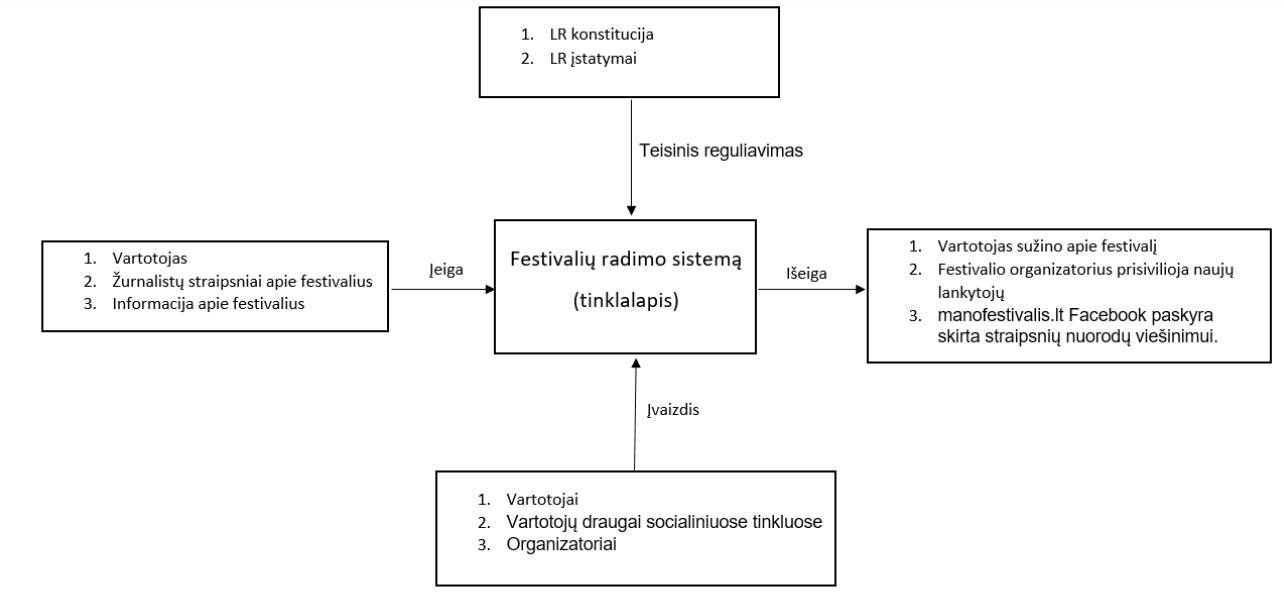
\includegraphics[scale=0.5]{img/geri/IsorineA}
    \label{img:uml0}
	\caption{Įeiga, išeiga ir reguliavimas}
\end{figure}
\noindent
Įeiga:
\begin{itemize}
\item Vartotojas - žmogus įsijungęs svetainę, norintis gauti informaciją, apie buvusius ir ateinančius festivalius;
\item Žurnalistų straipsniai apie festivalius;
\item Informacija apie festivalius - tiekiama festivalio organizatorių arba surandama administratorių. Sudedamosios dalys: festivalio tinklalapis, bilietų pardavėjas, festivalio vieta, laikas, nuotraukos susijusios su festivaliu(plakatai), festivalio aprašas.
\end{itemize}
Išeiga:
\begin{itemize}
\item Vartotojas sužino apie festivalį;
\item Festivalio organizatorius prisivilioja naujų lankytojų;
\item Nuorodos į tinklalapio straipsnius skirtos dalintis “Facebook” paskyroje
\end{itemize}
Įvaizdžio esybės:
\begin{itemize}
\item Vartotojai;
\item Vartotojų draugai socialiniuose tinkluose;
\item Festivalių organizatoriai
\end{itemize}
Teisinis reguliavimas:
\begin{itemize}
\item Lietuvos Respublikos konstitucija;
\item Lietuvos Respublikos įstatymai;
\end{itemize}
\subsection{Aprašas}



“Naujienų” skiltyje klientas mato paveikslėlius su straipsnių pavadinimais.
Paspaudus ant jų, pateikiamas straipsnis apie festivalį su galimybėmis dalintis juo socialiniuose tinkluose ir komentuoti. 

Skiltyje “Festivaliai” yra navigacijos dalis, kurioje galima pasirinkti festivalio kategoriją, likusioje skilties dalyje yra paveikslėlių (plakatų), kurie turi festivalio pavadinimą bei trumpą informaciją apie jį, kratinys. Paspaudus ant paveikslėlio, įkeliamas naujas puslapis, kuriame pateikiama informacija apie festivalio vietą (naudojant “Google Maps”), trumpa programa, bilietų kaina, nuorodos į oficialų tinklalapį ir pardavėjų puslapį. Yra galimybė pasidalinti informacija apie festivalį per “Facebook”, “Google+” ir “Twitter”. Šalia pateikiami naujausių festivalių, populiariausių festivalių bei panašių festivalių sąrašai. 

“Kalendoriaus” skiltyje tinklapio lankytojams pateikiamas kalendorius, kuriame festivaliai yra sužymėti pagal dienas.

“Žemėlapio”  skiltyje yra pateikiamas “Google Maps” žemėlapis, kuriame pažymėtos kai kurių (ne visų) festivalių vietos bei jų pavadinimai.
 
“Apie mus” skiltyje pateikiama informacija apie tinklapio sukūrimą, pasiūlymas paremti tinklalapį savo 2\% nuo pajamų mokesčių.
Yra atskira skiltis “Pranešk apie festivalį”, kuriame lankytojas gali nemokamai pateikti informacija apie festivalį nurodydamas pavadinimą, kategoriją, miestą, tikslų adresą, aprašymą, kainą, festivalio pradžią, pabaigą, festivalio logotipą, oficialų festivalio interneto puslapį, bilietų pirkimo puslapį, kontaktinį elektroninį paštą. 



\subsection{Metrikos}
\begin{longtable}{|p{0.2\linewidth}|p{0.2\linewidth}|p{0.2\linewidth}|p{0.15\linewidth}|p{0.15\linewidth}|} 
  \caption{Metrikos}\\
	\hline
	Metrikos & Matavimo vienetas & Kaip matuoti & Dabartinė reikšmė & Kritinė reikšmė \\
    \hline
    Vartotojų skaičius  & Žmonių, kurie dažnai naudojasi tinklalapiu, kiekis vienetais   & Suskaičiuoti, kiek žmonių įsijungia tinklalapį nors kartą per mėnesį  & 4 000 & 7 500 \\
	\hline
    Vartotojų aktyvumas  & 
Komentarų ir atsiliepimų, kurie prisideda prie svetainės ir festivalių informacijos gerinimo, kiekis vienetais
    & Suskaičiuoti, kiek iš viso yra komentarų ir atsiliepimų susijusių su svetainės veikimu ir tiekiama informacija  & 5 & 1000    \\
    \hline
    “Facebook” puslapio vertinimas žvaigždutėmis  & 
Žvaigždučių kiekis puslapyje
    & Patikrinti žvaigždučių skaičių “Facebook” puslapyje  & (nėra galimybės apskaičiuoti) & 4,8   \\
    \hline
Tinklalapio peržiūros  & 
Žmonių, kurie nors kartą buvo prisijungę į tinklalapį, kiekis vienetais
    & Suskaičiuoti individualius IP adresus  & 20 000 & 100 000   \\
    \hline
    Žmonių, potencialiai perkančių bilietą per nuoroda iš mūsų puslapio, kiekis   & 
Nuorodos į bilietų tiekėjo puslapį paspaudimų kiekis, vienetais 
    & Suskaičiuoti, kiek kartu paspausta nuoroda iš tam tikro festivalio  & (nėra galimybės apskaičiuoti) & 10   \\
    \hline
    Atsiliepimų kiekis po festivalio   & 
Po festivalių aprašymais paliktų komentarų kiekis vienetais 
    & Suskaičiuoti atsiliepimus apie festivalį  & 0 & 20   \\
    \hline
    Festivalių organizatorių kiekis kurie nori  patalpinti skelbimus   & Organizatorių, kurių festivalių informaciją talpiname, kiekis vienetais 
    & Suskaičiuoti visus organizatorius, kurie dalinasi ir trokšta dalintis informacija apie savo organizuojamus festivalius  & 45 & 100   \\
    \hline
    Talpinamų skelbimų kiekis   & 
Skirtingų festivalių skelbimų kiekis vienetais 
    & Suskaičiuoti kiek iš viso turime skirtingų patalpintų festivalių  & >2000 & 5000   \\
    \hline 
    Kiekis organizatorių perkančių reklamą pas mus   & 
Organizatorių kiekis vienetais
    & Suskaičiuoti kiek organizatorių perka reklamą  & 0 & 16   \\
    \hline
    Kiekis žmonių, kurie mėgsta mūsų puslapį per “Facebook”   &  “Like” kiekis vienetais “Facebook” puslapyje & Patikrinti “Like” skaičių “Facebook” puslapyje  & 6168 & 50 000   \\
    \hline
    2\% pajamų  mokesčiu paramos  kiekis & Vartotojų kiekis kurie skyrė 2\% & Peržvelgti kiek vartotojų skyrė savo 2\%  & 10 & 100   \\ \hline
\end{longtable}

\section{Vidinė proceso analizė}
\subsection {Dalykinės srities statinė struktūra}
Išanalizavę išorinę “manofestivalis.lt” struktūrą, mes padarėme spėjimą kaip viskas veikia tinklalapio viduje (baltąją dėžę).
Pagal dalykinės srities statinę strukūrą (pav. /?Number?/) matyti pagrindinės klasės: sistemos savininkas, tinklalapis, festivalio aprašymo puslapis,
 socialiniai įskiepiai (“G+1”, “Tweet”, “Like” mygtukai, “Facebook” komentarų erdvė), festivalių duomenų bazė, vartotojas, administratorius, žurnalistas, festivalio organizatorius,
 informacija apie festivalį (“Google Maps” žemėlapyje pavaizduota festivalio vieta, festivalio data, festivalio nuotraukos, festivalio aprašas, nuorodos į oficialų festivalio tinklalapį bei bilietų pardavimo puslapį). 

\textbf{Tinklalapis} sieja informacija ir vartotojus. Jame talpinami susisteminti festivalių puslapiai ir straipsniai, leidžiantys vartotojui ieškoti festivalių. Tinklalapį finansuoja sistemos savininkas, prižiūri ir tvarko sistemos administratorius.

\textbf{Festivalio aprašymo puslapis} talpina socialinių tinklų įskiepius ir informacija apie festivalį, kurią gauna per festivalių duomenų bazę.  

\textbf{Tinklalapio vartotojas} yra informacijos ieškotojas. Jis naudojasi tinklalapiu norėdamas sužinoti informaciją apie festivalius ir skaityti straipsnius apie festivalius. Jis gali komentuoti apie festivalius ir straipsnius komentarų erdvėje prisijungęs prie savo “Facebook” paskyros, dalintis informacija naudodamas socialinių tinklų įskiepius. Taip pat vartotojas gali rašyti atsiliepimus apie patį tinklapį administratoriui.

\textbf{Socialinio tinklalpio įskiepis} leidžia vartotojui reaguoti į pateikta informaciją. “Like”, “Tweet”, “G+1” mygtukai  ir “Facebook” komentarų erdvė leidžia pasidalinti ar išreikšti savo nuomonę, jei jis naudojasi atitinkamo socialinio tinklo paslaugomis.

\textbf{Straipsnio puslapis} yra atskiras puslapis, kuriame bandoma sudominti vartotoją festivaliu. Jis savyje talpina socialinius įskiepius leidžiančius vartotojui vertinti ir dalintis straipsniu.

\textbf{Administratorius} yra pagrindinis tinklalapio veiklos prižiūrėtojas.
Jis moderuoja komentarų erdvę - šalina netinkamus komentarus, prižiūri festivalio organizatorių pateikiamą informaciją (ar ši yra teisinga), jei reikia susisiekia su organizatoriumi dėl papildomos informacijos, užtikrina sklandų puslapio veikimą (prižiūri techninę tinklalapio dalį) ir pats suradęs festivalį, kurio skelbimo dar nėra tinklalapyje, gali patalpinti informaciją apie jį.

\textbf{Sistemos savininkas} gali sutapti su administrariumi ar žurnalistu arba kitiems paskirti šias pareigas.

\textbf{Festivalių organizatorius} yra asmuo rengiantis festivalį bei turintis oficialią informaciją. Norėdamas populiarinti savo festivalį jis gali pateikti informaciją apie savo festivalį, kurią įvertinęs administratorius patalpins tinklalapyje.

\textbf{Žurnalistas} stengiasi populiarinti festivalius ir tinklalapį. Jis gali patalpinti į tinklalapį parašytus ar surastus straipsnius.

\textbf{Festivalių duomenų bazė kaupia} informaciją apie festivalius.

\textbf{Informacija apie festivalius} - festivalio aprašymas, data, vieta, kaina, oficialus puslapis ir bilietų pardavėjo puslapis (jeigu yra).

\textbf{“Facebook” komentarų erdvė} yra socialinių tinklų įskiepis, kuriame vartotojai gali išsakyti savo mintis naudomi “Facebook” paskyrą.

\begin{figure}[H]
    \centering
    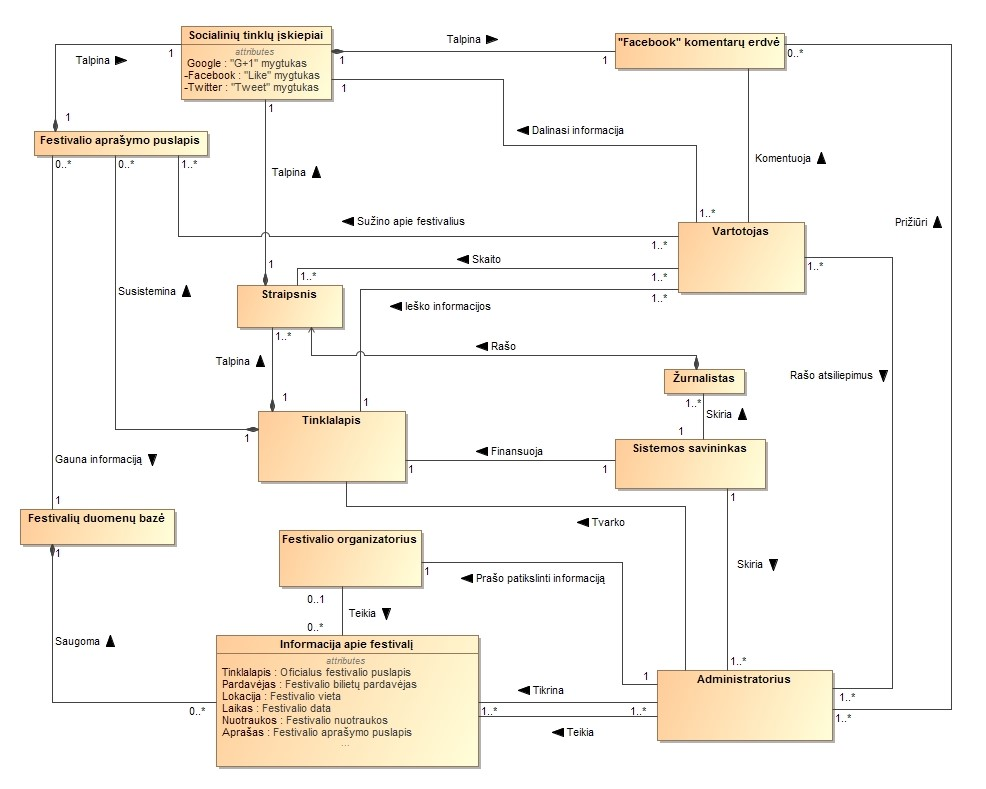
\includegraphics[scale=0.45]{img/geri/Statine_struktura}
    \label{img:uml1}
	\caption{Sistemos statinė struktūra}
\end{figure}

\subsection {Užduotys}

\begin{figure}[H]
    \centering
    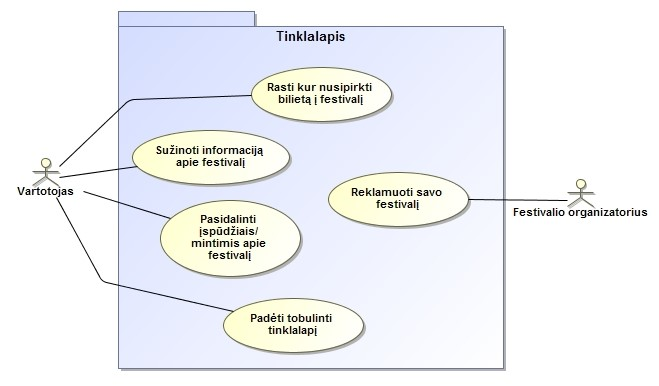
\includegraphics[scale=0.5]{img/geri/UzduotysIS}
    \label{img:uml2}
	\caption{Išorinių agentų užduotys}
\end{figure}

\begin{itemize}
\item Vartotojas yra agentas, kurio vienas iš siekių yra ieškoti informacijos apie festivalius (arba tiesiog ieškoti naujų festivalių, kuriuose galėtų sudalyvauti), tačiau vartotojas žinodamas, kokiame festivalyje nori dalyvauti jis nebūtinai žinos, kur gali nusipirkti bilietą, todėl tai yra jo antroji užduotis. Sudalyvavę festivalyje arba tiesiog tinklalapio vartotojai gali išsakyti savo nuomonę apie pasirinktajį festivalį komentarų erdvėje. Beje, vartotojas norėdamas prisidėti prie svetainės gyvavimo bei augimo gali pasidalinti savo idėjomis su administratoriumi.
\item Festivalio organizatoriaus pagrindinė užduotis yra platinti bei reklamuoti savo festivalį tam, kad kuo daugiau žmonių sudalyvautų jo ruošiamame renginyje.
\end{itemize}

\begin{figure}[H]
    \centering
    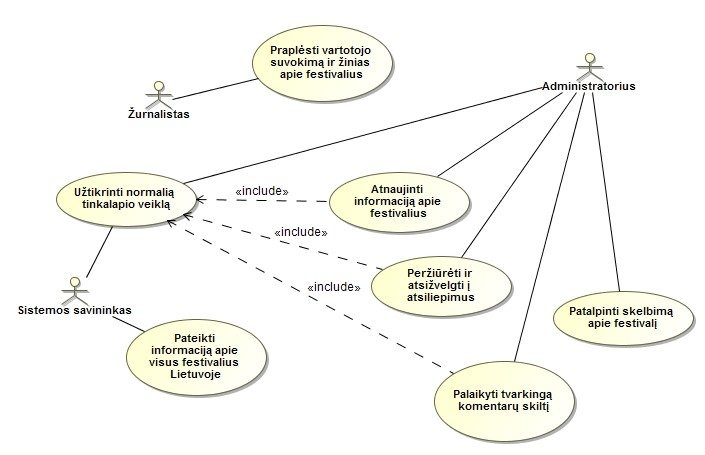
\includegraphics[scale=0.6]{img/geri/UzduotysVID}
    \label{img:uml3}
	\caption{Vidinių agentų užduotys}
\end{figure}

\begin{itemize}
\item Administratoriaus užduotys kyla iš to, kad jis siekia palaikyti normalią tinklalapio veiklą ir augimą (naujų festivalių skelbimų kėlimą). Tad, administratorius turi prižiūrėti komentarų erdvę tam, kad nebūtų netinkamų komentarų (spam, patyčių ir t.t), pasikeitus informacijai apie festivalius ją atnaujinti, kad nebūtų apgaulingos (netikslios) reklamos bei atsižvelgti į vartotojo pasiūlymus kaip tobulinti svetainės darbą, išsidėstymą. Tačiau vienas iš svarbiausių užduočių yra kelti naujus skelbimus į tinklalapį, kad jame nuolatos būtų aktuali informacija.
\item Sistemos savininkas siekia pateikti lengvai vartotojui prieinamą informaciją apie visus Lietuvos festivalius viename tinklalapyje, kad jam ieškojimas reikalingos informacijos būtų kuo trumpesnis. Beje, sistemos savininkas prižiūri, kad administratorius atliktų savo darbą ir tinklalapis veiktų puikiai.
\item Žurnalistas siekia praplėsti vartotojų žinias ir suvokimą apie festivalius bei sudominti tinklalapio turiniu, nes per straipsnius pristato pagrindinę tinklalapio temą - festivalis.
\end{itemize}

\subsection {Užduočių vykdymo scenarijai}

Agentas norėdamas atlikti savo užduotis turi atlikti tam tikrus žingsnius.

\subsubsection{Išorinių agentų užduotys} 
\begin{figure}[H]
    \centering
    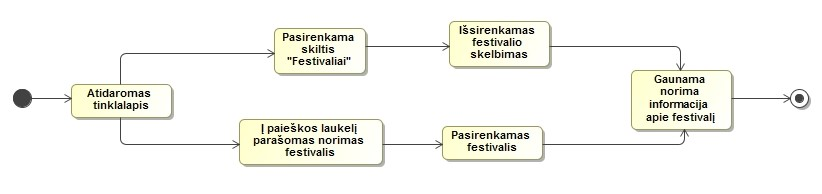
\includegraphics[scale=0.55]{img/geri/klientasInfo}
    \label{img:uml3_5}
	\caption{Vartotojas ieško informacijos}
\end{figure}

Vartotojas norėdamas rasti daugiau informacijos:
\begin{itemize}
\item Atidaro tinklalapį.
\item Pirmas atvejis:
\begin{itemize}
\item vartotojas navigacijos dalyje pasirenka skiltį “Festivaliai”;
\item festivalių skelbimų kratinyje išsirenka festivalį, apie kurį nori sužinoti daugiau.
\end{itemize}
\item Antras atvejis:
\begin{itemize}
\item į paieškos laukelį įvedamas norimo festivalio pavadinimas;
\item pasirenkamas norimas festivalis.
\end{itemize}
\item Atsidaro naujas tinklalapio puslapis su informacija apie norimą festivalį.
\end{itemize}

\begin{figure}[H]
    \centering
    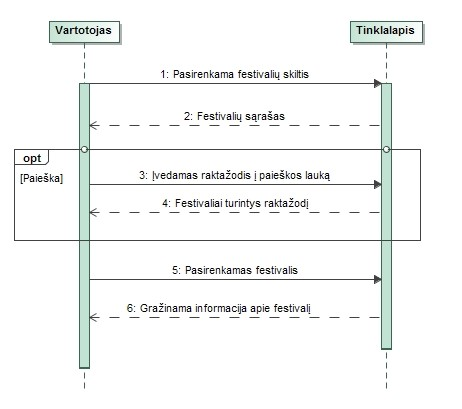
\includegraphics[scale=0.7]{img/geri/_klientasInfo}
    \label{img:uml4}
	\caption{Informacijos gavimo sekų diagrama}
\end{figure}

Vartotojas norėdamas sužinoti informaciją apie festivalį, tinklalapyje pasirenka festivalių skiltį. Tinklalapis pateikia festivalių sąrašą. Vartotojas gali paieškos laukelyje įvesti norimo festivalio raktažodį ir tinklalapis pateikia tik tuos festivalius, kurie turi tą raktažodį. Arba vartotojas gali iš festivalių sąrašo pasirinkti jį dominantį festivalio skelbimą ir tinklalapis gražins informaciją apie jį.

\begin{figure}[H]
    \centering
    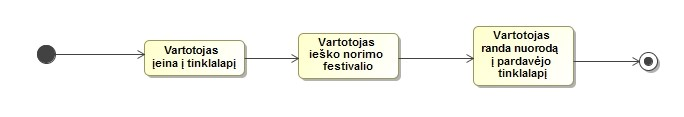
\includegraphics[scale=0.6]{img/geri/klientasBilietas}
    \label{img:uml5}
	\caption{Vartotojas ieško kur nusipirkti bilietą}
\end{figure}

Vartotojas norėdamas nusipirkti bilietą į festivalį:
\begin{itemize}
\item Atidaro tinklalapį.
\item Randa norimą festivalį.
\item Festivalio aprašyme randa nuorodą į pardavėjo tinklalapį, kuriame įsigyja bilietą.
\end{itemize}

\begin{figure}[H]
    \centering
    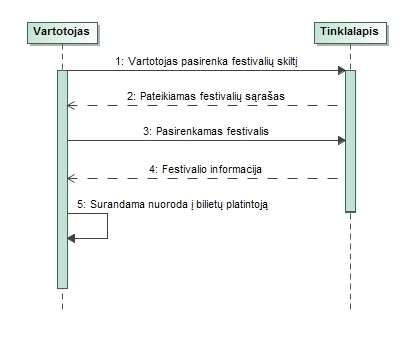
\includegraphics[scale=0.7]{img/geri/_klientasBilietas}
    \label{img:uml6}
	\caption{Bilietų ieškojimo sekų diagrama}
\end{figure}

Vartotojas norėdamas rasti, kur nusipirkti bilietą, tinklalapyje pasirenka festivalių skiltį. Tinklalapis pateikia festivalių sąrašą, iš kurio vartotojas gali pasirinkti norimą festivalį. Tada tinklalapis vartotojui pateikia festivalio informaciją - vartotojas šioje informacijoje suranda nuorodą į bilietų platintoją.

\begin{figure}[H]
    \centering
    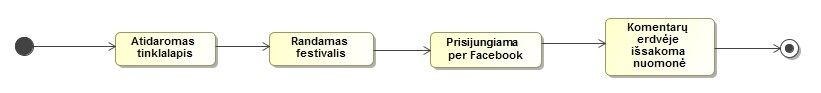
\includegraphics[scale=0.5]{img/geri/klientasmintis}
    \label{img:uml7}
	\caption{Vartotojai komentuoja festivalius}
\end{figure}

Vartotojas norėdamas pasidalinti įspūdžiais (mintims) apie festivalį:
\begin{itemize}
\item Atidaro tinklalapį.
\item Suranda norimą festivalį.
\item Prisijungęs prie “Facebook” paskyros, komentarų erdvėje išsako savo nuomonę.
\end{itemize}
\begin{figure}[H]
    \centering
    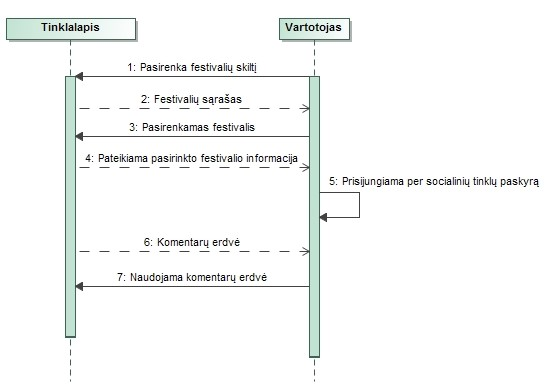
\includegraphics[scale=0.7]{img/geri/_klientasKom}
    \label{img:uml8}
	\caption{Komentavimo sekų diagrama}
\end{figure}

Vartotojas norėdamas pasidalinti įspūdžiais ar mintimis apie festivalį gali tinklalapyje pasirinkti festivalių skiltį. Tinklalapis jam pateikia festivalių sąrašą, iš kurio vartotojas pasirenka festivalį. Tada tinklalapis vartotojui pateikia pasirinktojo festivalio informaciją. Vartotojas prisijungia prie savo socialinių tinklų paskyros ir tada tinklalapis leidžia vartotojui naudotis komentarų erdve.

\begin{figure}[H]
    \centering
    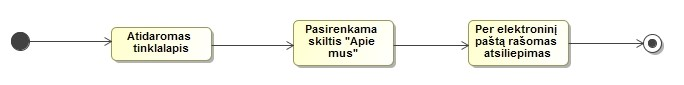
\includegraphics[scale=0.7]{img/geri/klientasKom}
    \label{img:uml9}
	\caption{Vartotojas teikia atsiliepimus}
\end{figure}

Vartotojas norėdamas prisidėti prie tinklalapio tobulinimo:
\begin{itemize}
\item Atidaro tinklalapį.
\item Navigacijos dalyje pasirenka skiltį “Apie mus” bei poskiltį “Kontaktai”.
\item Šioje skiltyje randa tinklalapio informacinio elektroninio pašto adresą, kuriuo išsiunčia atsiliepimą apie tinklalapį.
\end{itemize}

\begin{figure}[H]
    \centering
    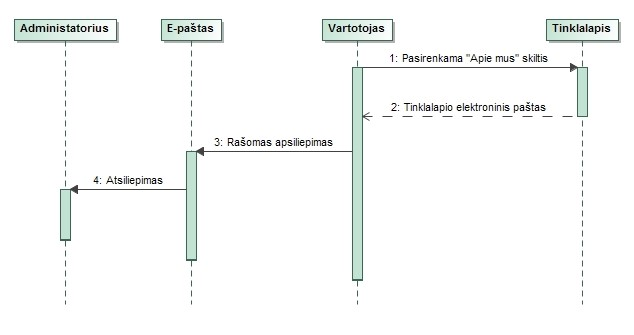
\includegraphics[scale=0.7]{img/geri/_klientasmintis}
    \label{img:uml10}
	\caption{Atsiliepimų sekų diagrama}
\end{figure}

Vartotojas norėdamas padėti tobulinti tinklalapį , jame pasirenka skiltį “Apie mus”, toje skiltyje randa tinklalapio elektroninį paštą. Tada vartotojas naudodamasis savo elektroniniu paštu parašo atsiliepimą į tinklalapio elektroninį paštą. Administratorius gauną elektroninį laišką su vartotojo atsiliepimu apie tinklalapį. 

\begin{figure}[H]
    \centering
    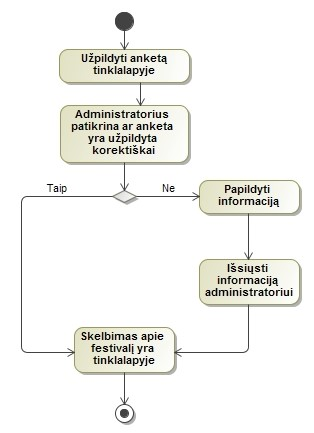
\includegraphics[scale=0.7]{img/geri/festivalOrg}
    \label{img:uml11}
	\caption{Organizatorius nori patalpinti skebimą}
\end{figure}

Festivalio organizatorius norėdamas reklamuoti savo festivalį:
\begin{itemize}
\item Užpildo anketą tinklalapyje.
\item Jei jis gauna puslapio administratoriaus pranešimą dėl netinkamos informacijos, festivalio organizatorius informaciją turi patikslinti ir/arba papildyti, nes kitaip administratorius informacijos į tinklalapį neįkels.
\end{itemize}

\begin{figure}[H]
    \centering
    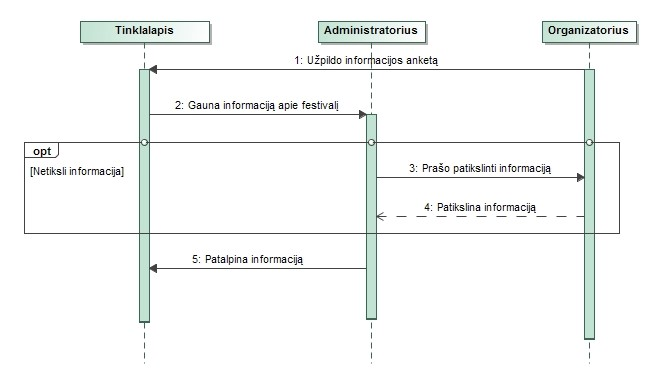
\includegraphics[scale=0.7]{img/geri/_Organizatorius}
    \label{img:uml12}
	\caption{Patalpinimo sekų diagrama}
\end{figure}

Festivalio organizatorius tinklalapyje užpildo informacijos anketą. Tada administratorius gauna informaciją apie festivalį . Jeigu festivalio organizatoriaus informacija yra netiksli arba neteisinga - administratorius parašo ją patikslinti, tuomet festivalio organizatorius patikslina informaciją. Ir tada administratorius patalpina informaciją (festivalio skelbimą) į tinklalapį.

\subsubsection{Vidinių agentų užduotys} 

\begin{figure}[H]
    \centering
    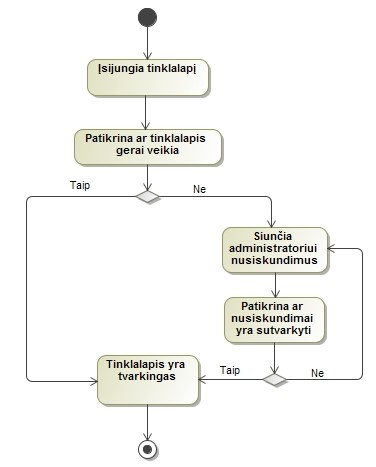
\includegraphics[scale=0.7]{img/geri/sistemosSav}
    \label{img:uml13}
	\caption{Savininkas tikrina tinklalapio tvarkingumą}
\end{figure}

Sistemos savininkas norėdamas užtikrinti normalią tinklapio veiklą:
\begin{itemize}
\item Įjungia tinklalapį.
\item Tinklalapio veikimo patikrinimas: 
\begin{itemize}
\item tinklalapis greitai (max 5s) pasikrauna, kad vartotojas kuo efektyviau galėtų išnaudoti tinklalapį ir kuo daugiau laiko praleistų jame kažką veikdamas, o ne laukdamas, kad pasikraus;
\item tinklalapio informacija turi būti nuolatos atnaujinama ir patikrinama, kad nebūtų apgaulingos reklamos ir kad neprarastume vartotojo pasitikėjimo tinklalapio informacijos teisingumu;
\item komentarų erdvėje nėra šlamšto (spam), įžeidžiančių komentarų.
\end{itemize}
\item Jeigu kažkas yra blogai, nusiskundimas yra siunčiamas administratoriui: 
\begin{itemize}
\item jis privalo sutvarkyti sistemos savininko nusiskundimus ir tada tinklalapis vėl tampa tvarkingu ir normaliai veikiančiu;
\item jeigu ne - sistemos savininkas patikslina savo nusiskundimą tam, kad adminsitratorius geriau suvoktų, ką reikia pakeisti ar pataisyti.
\end{itemize}
\end{itemize}

\begin{figure}[H]
    \centering
    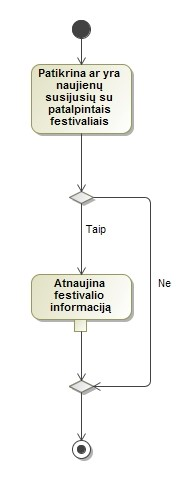
\includegraphics[scale=0.7]{img/geri/adminAtnaujinti}
    \label{img:uml14}
	\caption{Administratorius atnaujina fesitvalio informaciją}
\end{figure}

Administratorius, norėdamas atnaujinti informaciją apie festivalį:
\begin{itemize}
\item Suranda patikimų naujienų apie festivalius, kurių informacija jau patalpinta tinklalapyje, arba festivalio organizatorius praneša apie pakitusią festivalio informaciją.
\item Jeigu yra pakitus festivalio informacija, ją atnaujina, kad vartotojas galėtų rasti tik tikslią informaciją.  
\end{itemize}

\begin{figure}[H]
    \centering
    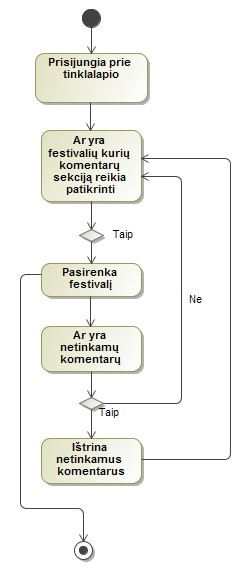
\includegraphics[scale=0.7]{img/geri/adminKom}
    \label{img:uml15}
	\caption{Administratorius palaiko tvarkingą komentarų skiltį}
\end{figure}

Administratorius, norėdamas palaikyti tvarkingą komentarų skiltį:
\begin{itemize}
\item Prisijungia prie tinklalapio.
\item Patikrina ar yra netikrintų festivalių komentarų sekcijų:
\begin{itemize}
\item Jeigu yra, pasirenka festivalį;
\item Patikrina ar yra netinkamų komentarų:
\begin{itemize}
\item Patyčių,
\item Diskriminacijos,
\item Neatitinkančių temos,
\item Prieštarajančių Lietuvos įstatymams ir “Facebook” taisyklėms.
\end{itemize}
\item Pašalina netinkamus komentarus.	
\end{itemize}
\end{itemize}

\begin{figure}[H]
    \centering
    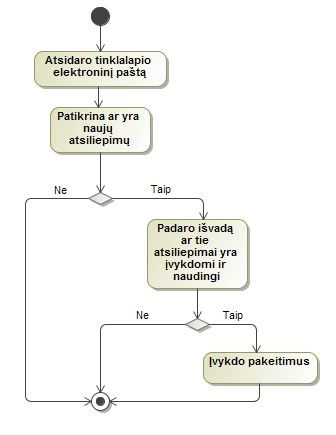
\includegraphics[scale=0.7]{img/geri/adminFeed}
    \label{img:uml15_5}
	\caption{Administratorius peržiūri atsiliepimus}
\end{figure}

Administratorius norėdamas peržiūrėti vartotojų atsiųstus atsiliepimus:
\begin{itemize}
\item Atsidaro informacinį tinklalapio elektroninį paštą.
\item Patikrina ar yra naujų atsiliepimų iš vartotojų.
\item Jeigu yra naujų, tuomet:
\begin{itemize}
\item Įvertina ar atsiliepimai yra naudingi tinklalapiui ir ar pasiūlymai yra įvykdomi;
\item Jeigu taip, įvykdo pakeitimus.
\end{itemize}
\end{itemize}

\begin{figure}[H]
    \centering
    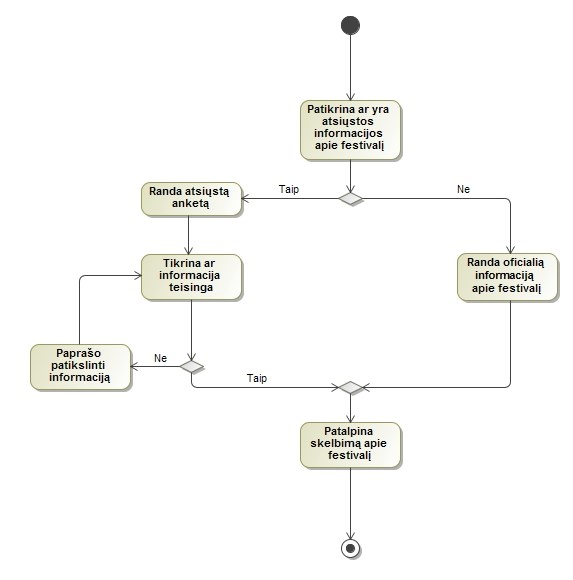
\includegraphics[scale=0.7]{img/geri/adminSkelb}
    \label{img:uml16}
	\caption{Administratorius įkelia skelbimą į FDB}
\end{figure}

Administratorius norėdamas patalpinti į FDB naują skelbimą apie festivalį:
\begin{itemize}
\item Prisijungia prie FDB.
\item Jei yra pateikta nauja arba patikslinta informacija apie festivalius:
\begin{itemize}
\item Tikrina ar informacija yra teisinga.
\item Jeigu informacija netinkama, prašo festivalio organizatoriaus patikslinti informaciją.
\item Jeigu informacija teisinga, patalpina skelbimą apie festivalį į tinklalapį.
\end{itemize}
\item Jei naujos informacijos nepateikta:
\begin{itemize}
\item Ieško naujos informacijos.
\item Rastą informaciją, talpina į tinklalapį.
\end{itemize}
\end{itemize}

\begin{figure}[H]
    \centering
    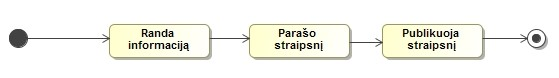
\includegraphics[scale=0.7]{img/geri/zurnalistas}
    \label{img:uml17}
	\caption{Žurnalistas publikuoja straipsnį}
\end{figure}

Žurnalistas norėdamas praplėsti vartotojo žinias ir suvokimą apie festivalius:
\begin{itemize}
\item Randa informaciją apie festivalius.
\item Parašo straipsnį remdamasis rasta informacija.
\item Publikuoja straipsnį į tinklalapį.
\end{itemize}

\subsection{Dalykinės srities dinaminė struktūra}
\begin{figure}[H]
    \centering
    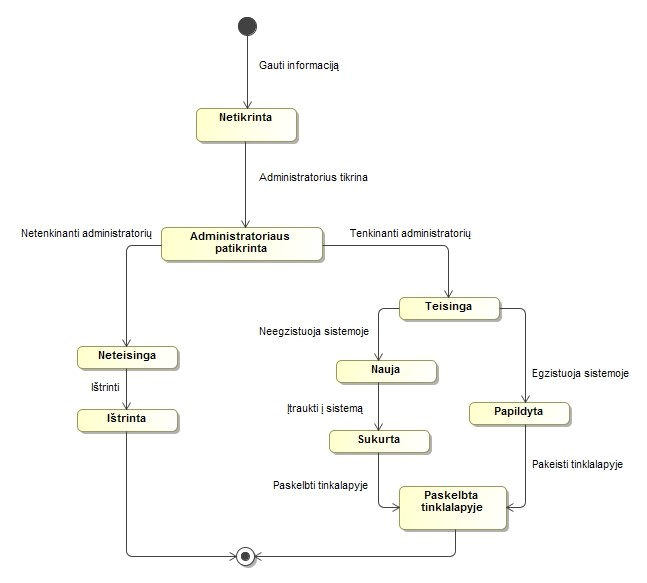
\includegraphics[scale=0.7]{img/geri/Informacija_Busenos.jpg}
    \label{img:uml18}
	\caption{Festivalio informacijos būsenos}
\end{figure}
Informacija apie festivalius gali būti įvairių būsenų: netikrinta, administratoriaus patikrinta, teisinga, neteisinga, nauja, sukurta, papildyta, paskelbta tinklalapyje, ištrinta. Kai festivalio organizatorius užpildo tinklalapyje esančią anketą, ji yra gaunama į informacija apie festivalius dalį ir turi būseną netikrinta. Kai administratorius patikrina informaciją apie festivalį, ji įgauna būseną administratoriaus patikrinta. Po patikrinimo informacija gali:
\begin{itemize}
\item netenkinti administratoriaus (šlamštas, reklama, nepagarba kitiems ir t.t.) ir turėti būseną neteisinga, o po to, būna ištrinama ir taip įgauna būsena ištrinta;
\item tenkinti administratorių ir turėti būseną teisinga. Festivalio skelbimas gali jau egzistuoti sistemoje, bet nebūti paskelbtas dėl to, kad yra reikalingas papildymas ir ši nauja informacija yra jau esančio festivalio informacijos papildymas ir taip informacija apie festivalius įgauna būseną papildyta. Tačiau informacijos gali ir nebūti sistemoje todėl ji įgauna būseną nauja. Ir administratoriui įtraukus ją į sistemą ji gauna būseną sukurta. 
\end{itemize}
Abiem atvejais informacija apie festivalius (ar papildyta, ar sukurta) pasiekia būseną paskelbta tinklalapyje.

\begin{figure}[H]
    \centering
    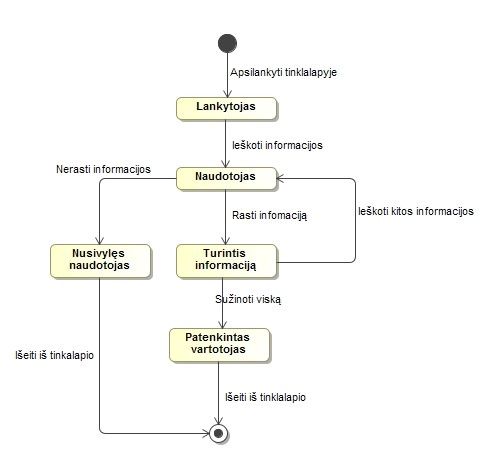
\includegraphics[scale=0.7]{img/geri/Vartotojas_Busenos.jpg}
    \label{img:uml19}
	\caption{Vartotojo būsenos}
\end{figure}
Vartotojas gali būti: lankytojas; naudotojas; naudotojas, turintis informaciją; nusivylęs naudotojas; patenkintas vartotojas. Kai vartotojas apsilanko tinklalapyje jis gauna būseną lankytojas. Bet kai vartotojas ne vien apsilanko, bet ir ieško informacijos, jis tampa naudotoju. Neradęs jam reikalingos informacijos naudotojas įgauna būseną nusivylęs naudotojas. Kai naudotojas randa informaciją jis tampa turintis informaciją, bet jei jis nerado visos jam reikiamos informacijos jis gali toliau ieškoti ir vėl tampa naudotoju. Jeigu naudotojas randa visą jam norimą informaciją jis įgauna būseną patenkintas vartotojas.

\begin{figure}[H]
    \centering
    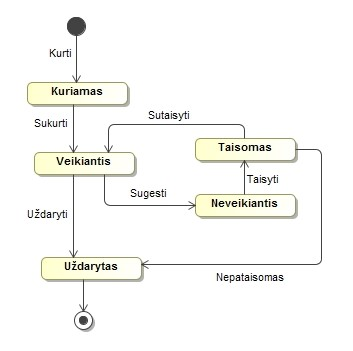
\includegraphics[scale=0.8]{img/geri/Tinkalalio_Busenos.jpg}
    \label{img:uml20}
	\caption{Tinkalalio būsenos}
\end{figure}
Tinklalapis gali būti: kuriamas, veikiantis, neveikiantis, taisomas, uždarytas. Jeigu tinklalapis neveikia dėl serverio talpintojų problemų arba dėl sistemos klaidų jis įgauna būseną neveikiantis. Pradėjus taisyti neveikiantis tinklalapis tampa taisomu. Pavykus sutaisyti tinklalapis grįžta į normalią būseną - veikiantis. Dėl finansų stygiaus arba populiarumo stygiaus tinklalapis gali tapti uždarytu.

\section{Analizės rezultatai}
\begin{longtable}{|p{0.45\linewidth}|p{0.45\linewidth}|} 
  \caption{SSGG}\\
  \hline
  \textbf{Stiprybės}
  \begin{itemize}
	\item Yra informatyviausias tinklalapis apie festivalius Lietuvoje.
	\item Festivalių organizatoriai gali laisvai reklamuoti renginius. Virš 6100 žmonių yra pamėgę "manofestivalis.lt".
	\item Festivaliai turi lygias galimybes - jie rodomi taip pat, neatsižvelgiant į jų populiarumą.
  \end{itemize}
  &
  \textbf{Silpnybės}
  \begin{itemize}
	\item Festivalių skelbimai pateikiami kaip neorganizuotas paveikslėlių kratinys.
	\item Pasenę festivalių skelbimai nėra išimami iš bendros ateinančių festivalių erdvės, todėl vartotojui yra sukuriama iliuzija, kad Lietuvoje atitinkamu metu vyksta daug festivalių.
	\item Festivalių ieškojimas yra neefektyvus dėl per didelio skaičiaus senų festivalių.
	\item Vartotojai beveik nesinaudoja komentarų erdve. Net didžiausi Lietuvos festivaliai susilaukia tik po vieną komentarą.
	\item Administratorius nebūtinai tinkamai atlieka savo darbą, kadangi sistemos savininkas ne visą laiką jį kontroliuoja.
	\item Festivalių skelbimas gali būti patalpintas tinklalapio administratoriaus be festivalio organizatorius žinios.
	\item Festivalių organizatoriai tinklalapio nemato kaip tikslingos vietos reklamuotis dėl per mažo populiarumo.
	\item Tinklalapis negeneruoja lėšų.
  \end{itemize}\\
  \hline
  \textbf{Galimybės}
  \begin{itemize}
	\item Sukurti vartotojui patogią festivalių rikiavimo ir rūšiavimo sistema pagal datą, kainą, miestą, kad vartotojas lengvai pasiektų reikalingą informaciją.
	\item Platesnis tinklalapio interaktyvumas - žmonės galės patogiau išreikšti savo nuomonę ir planuotis į kokius festivalius nori nueiti.
	\item Patobulinti komentarų erdvę, kad žmonės galėtų lengviau susipažinti su kitais festivalių dalyviais.
	\item Festivaliai galėtų išsipirkti savo  skelbimams specialias galimybes taip remdami tinklalapio plėtimąsi.
	\item Sukurti marketingo komanda, kuri siektų išpopuliarinti tinklalapį tam, kad festivalių organizatoriai norėtų dėti savo skelbimus į tinklalapį.
  \end{itemize}
  &
  \textbf{Grėsmės}
  \begin{itemize}
	\item Tinklalapio išlaikymas priklauso nuo vartotojų noro skirti savo lėšas.
	\item Dėl didelio senų festivalių kiekio festivaliai gali netilpti duomenų bazėje.
	\item Kiti tinklalapiai gali aplenkti savo populiarumu ir ryšiais su organizatoriais.
	\item Serveris gali neatlaikyti lankytojų skaičių.
	\item Dėl mūsų tinklalapyje naudojamų socialinių tinklų įskiepių mes prarandame komentarų ir vertimų kontrolę. / Sklandus vertinimų ir komentarų erdvės veikimas yra priklausomas nuo socialinių tinklų veikimo.
  \end{itemize}\\
  \hline
\end{longtable}

\section{Verslo proceso tobulinimo strategija}
Pagrindinis mūsų tikslas yra sukurti geresnę sistemą negu, kad jau yra sukurta. Šito mes sieksime padidindami tinklalapio interaktyvumą (vartotojas galės susikurti paskyrą, o prisijungęs turės daugiau galimybių (pateikta žemiau), palengvinsime festivalių paiešką), populiarinti tinklalapį Lietuvos mastu (stengtis, kad daugiau Lietuvos gyventojų žinotų bei naudotųsi tinklalapiu, festivalių organizatoriai siektų reklamuotis tinklalapyje), sukursime galimybę tinklalapiui finansuoti save, palengvinsime tinklalapio administratoriaus darbą.

Mūsų vizija yra padidinti žmonių aktyvumą bei kultūrinį suvokimą.
Mūsų misija yra palengvinti festivalių informacijos pasiekiamumą bei suprantamumą.
\begin{itemize}
\item Paskatinti vartotoją sugrįžti į svetainę:
	\begin{itemize}
    \item Padaryti galimybę vartotojui susikurti paskyrą tinklalapyje arba prisijungti su turima socialinių tinklų paskyra (“G+”, “Facebook”) ;
    \item Vartotojas susikūręs paskyrą galėtų:
        \begin{itemize}
        \item kalendoriuje pasižymėti festivalius, kuriuose nori sudalyvauti;
        \item užsiprenumeruoti festivalių skelbimus (jeigu festivalio informacija yra atnaujinama vartotojas bus perspėjamas);
        \item likus 3 dienoms iki festivalio vartotojas, jeigu yra pasižymėjęs kalendoriuje arba užsiprenumeravęs, būtų perspėtas apie meteorologines sąlygas festivalio dienomis;
        \item vartotojai norintys dalyvauti tame pačiame festivalyje galėtų tarpusavyje bendrauti atskiroje diskusijų erdvėje;
        \item rašyti atsiliepimus apie festivalius tam skirtoje tinklalapio erdvėje;
        \end{itemize}
    \end{itemize}
\item Patobulinti tinklalapio festivalių skitį:
    \begin{itemize}
    \item Leisti vartotojui pasirinkti kokius festivalius jis nori matyti: būsimus, vykstančius, praėjusius ar visus;
    \item Padaryti galimybę vartotojui pasirinkti pagal kokius kriterijus (datos intervalą, miestą, kainos intervalą) rūšiuoti festivalius, pasirinkti rikiavimą pagal pavadinimą, datą;
    \item Suvienodinti festivalių skelbimų dydį ir automatiškai surikiuoti chronologine tvarka;
    \end{itemize}
\item Sukurti galimybę tinklalapiui išlaikyti pačiam save:
    \begin{itemize}
    \item Kai kurias tinklalapio dalis paskirti mokamai festivalių reklamai (jų reklamos bus rodomos paskirtose tinklalapio dalyse iki išpirkto laiko pabaigos, ne vien festivalių skiltyje);
    \end{itemize}
\item Paskatinti vartotojus naudotis komentarų erdve:
    \begin{itemize}
    \item Pašalinti “Facebook” komentarų erdvę;
    \item Sukurti tinklalapio komentarų erdvę, kurioje prisijungę vartotojai galėtų komentuoti apie festivalį;
    \item Prisijungusiems tinklalapio vartotojams sukurti atskirą diskusijų erdvę bendrauti tarpusavyje apie festivalius, kuriuose dalyvaus;
    \end{itemize}
\item Didinti tinklalapio populiarumą:
    \begin{itemize}
    \item Sukurti marketingo komandą, kuri tiesiogiai susisiektų su festivalių organizatoriais ir pasiūlytų patalpinti jų skelbimą mūsų sistemoje, bendrautų dėl galimų bendrų akcijų;
    \item Marketingo komanda stengiasi sukurti bendruomenę “Facebook” tinklapyje ir taip paskatinti vartotojus naudotis tinklalapiu;
    \end{itemize}
\item Supaprastinti administratorius darbą:
    \begin{itemize}
    \item Sukurti “Admin panel” kuriame galima būtų matyti po praėjusio tikrinimo atsiradusius komentarus;
    \item Leisti vartotojams pranešti apie netinkamus komentarus ar netikslią informaciją;
    \end{itemize}
\end{itemize}

\section{Sistemos naudojimo scenarijus}
\subsection{Scenarijus}

Administratorius gali būti perspėtas dėl netinkamų komentarų bei matyti naujus komentarus.

\begin{figure}[H]
    \centering
    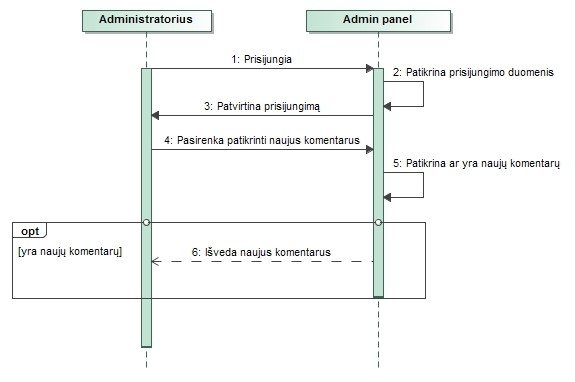
\includegraphics[scale=0.7]{img/geri/_adminNaujiCom}
    \label{img:uml21}
	\caption{"Admin panel" naudojimo sekų diagrama}
\end{figure}

Administratorius, norėdamas patikrinti komentarus, turės prisijungti prie “Admin panel” (jei prisijungimo duomenys teisingi, patvirtina prisijungimą), tada “Admin panel” išveda naujus komentarus administratoriui, o jis juos patikrina.

\begin{figure}[H]
    \centering
    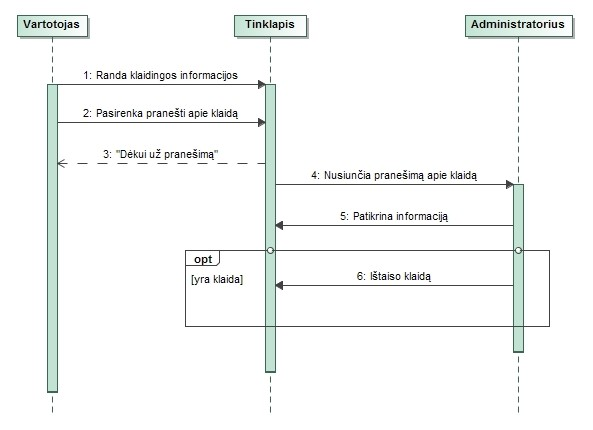
\includegraphics[scale=0.7]{img/geri/_adminError}
    \label{img:uml22}
	\caption{Netinkamos informacijos šalinimo sekų diagrama}
\end{figure}

Kad būtų lengviau surasti netinkama informaciją tinklapyje, vartotojas galės administratoriui apie tai pranešti. Vartotojas, radęs klaidingos informacijos festivalių skiltyje, praneša apie klaidą naudodamas tam skirtą funkciją ir automatiškai gauna žinutę su padėka. Pranešimas apie klaidą yra nusiunčiamas administratoriui, jis patikrina informaciją festivalių skiltyje ir, jeigu yra klaida, ją ištaiso.

Vartotojas yra dviejų būsenų: turintis tinklalapio paskyrą arba ne. Nuo to priklauso, kaip jis sąveikauja su sistema. 

\begin{figure}[H]
    \centering
    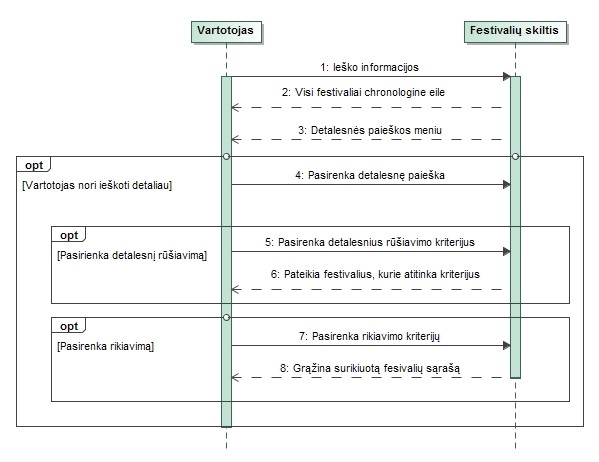
\includegraphics[scale=0.7]{img/geri/KlientPaieska}
    \label{img:uml23}
	\caption{Festivalių detalesnės paieškos sekų diagrama}
\end{figure}

Vartotojas, neturintis paskyros, gali ieškoti informacijos. Festivalių skiltis pateikia chronologiškai išrikiuotus festivalių skelbimus bei detalesnės paieškos meniu. Vartotojas, norintis ieškoti tam tikrų festivalių, gali pasirinkti rūšiavimo kriterijus (datos intervalą, miestą, kainos intervalą) bei pakeisti rikiavimo kriterijų (pagal pavadinimą arba datą). Festivalių skiltis grąžina sąrašą, išrūšiuota ir išrikiuota pagal vartotojo pageidavimus.

\begin{figure}[H]
    \centering
    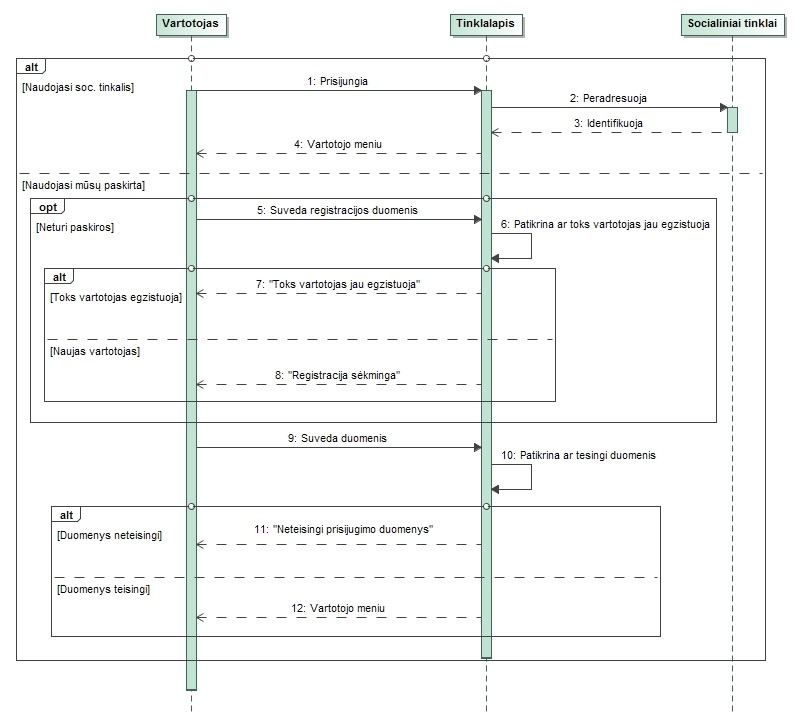
\includegraphics[scale=0.5]{img/geri/KlientPrisijungimas}
    \label{img:uml24}
	\caption{Vartotojo prisijungimo ir registracijos sekų diagrama}
\end{figure}

Vartotojas, norėdamas prisijungti prie tinklalapio, gali tai padaryti naudodamasis socialiniais tinklais (“G+”, “Facebook”). Tinklalapyje vartotojas pasirenka šią galimybę, iš tinklalapio yra nukreipiamas į socialinius tinklus ir indentifikuojamas. Tada tinklalapis rodo vartotojo meniu. Tačiau vartotojas gali prisijungti prie tinklalapio ir per vietinę paskyrą. Jeigu vartotojas neturi vietinės paskyros, pasirenka ją sukurti ir suveda visus reikiamus duomenis. Sistema patikrina ar toks vartotojas jau yra. Jeigu yra - išspausdina, kad toks vartotojas jau egzistuoja, jeigu ne - praneša, kad registracija sėkminga. Jei vartotojas jau turi paskyrą ir tiesiog nori prisijungti, suveda savo prisijungimo duomenis. Sistema patikrina, ar duomenys yra teisingi. Jeigu duomenys yra neteisingi, tinklalapis praneša, kad prisijungimo duomenys neteisingi. Jeigu teisingi, atidaro vartotojo meniu.

\begin{figure}[H]
    \centering
    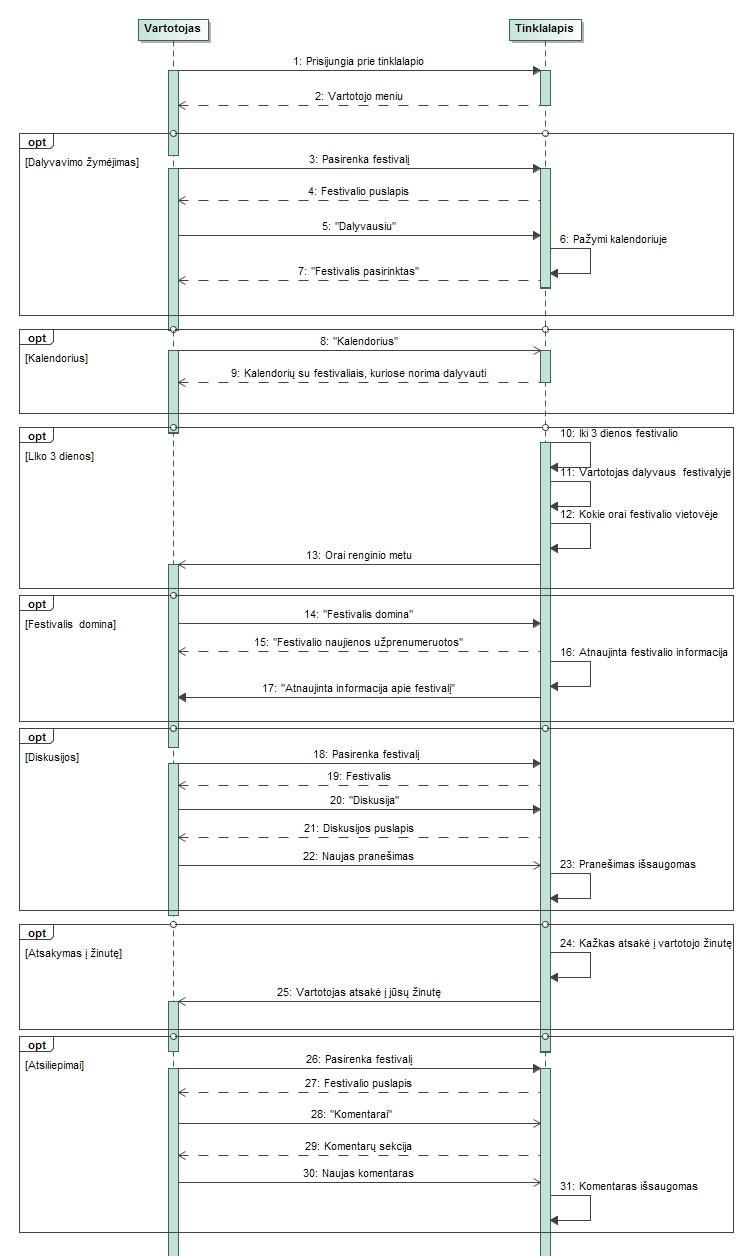
\includegraphics[scale=0.5]{img/geri/KlientFun}
    \label{img:uml25}
	\caption{Vartotojo galimybių sekų diagrama}
\end{figure}

Prisijungusiam vartotojui  tinklalapis rodo vartotojo meniu. Vartotojas kalendoriuje gali pažymėti, kad dalyvaus festivalyje: pasirenka festivalį, tinklalapis atidaro festivalio puslapį mūsų tinklalapyje. Kai vartotojas pasirenka “Dalyvausiu”, kalendoriuje pažymimos dienos, kuriomis vyks festivalis. Įvykdęs užduotį tinklalapis praneša vartotojui, kad festivalis pasirinktas. Jei vartotojas pasirenka “Domina”, tinklalapis praneša, kad festivalis yra sėkmingai užprenumeruotas. Vartotojas taip pat gali peržiūrėti savo kalendorių, kuriame jis yra pažymėjęs, kuriuose festivaliuose nori dalyvauti arba dalyvaus. Likus trims dienoms iki festivalių, kuriuos vartotojas yra pasižymėjęs kalendoriuje arba užsiprenumeravęs, vartotojas elektroniniu laišku yra perspėjamas apie meteorologinę situaciją festivalio vietoje. Vartotojas, tinklapyje pasirinkęs festivalį, gali patekti į diskusijos puslapį ir dalyvauti diskusijoje. Vartotojas galės rašyti naujus pranešimus ir tinklalapis juos saugos. Vartotojas yra perspėjamas, kai po jo pranešimu kitas vartotojas parašo komentarą. Atidaręs festivalio puslapį, registruotas vartotojas mato komentarų sekciją, kurioje gali reikšti savo nuomonę apie festivalį. Tinklalapis išsaugo komentarus sistemoje.

Marketingo komanda gali susisiekti su festivalių organizatoriais ir jiems pasiūlyti reklamuotis mūsų tinklalapyje bei per socialinius tinklalapius skelbti savo tinklalapį.

\begin{figure}[H]
    \centering
    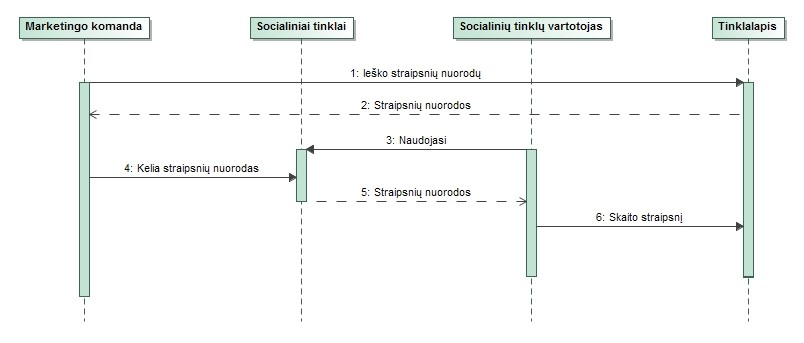
\includegraphics[scale=0.5]{img/geri/markfacebook}
    \label{img:uml26}
	\caption{Marketingo komandos reklamavimo sekų diagrama}
\end{figure}

Marketingo komanda norėdama rasti naujų vartotojų, kelia mūsų tinklalapio straipsnių nuorodas i socialinius tinklus, šias nuorodas randa socialinių tinklų vartotojai. Jie jas atsidaro ir įeina į tinklalapį.

\begin{figure}[H]
    \centering
    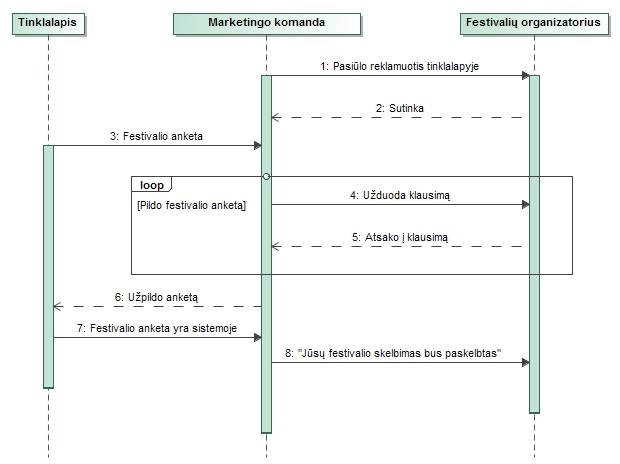
\includegraphics[scale=0.7]{img/geri/markIesko}
    \label{img:uml27}
	\caption{Susiekimo su orgamizatoriais sekų diagrama}
\end{figure}

Marketingo komanda, norėdama pasiūlyti festivalių organizatoriams skelbtis mūsų tinklalapyje, susisiekia su festivalių organizatoriais ir pasiūlo reklamuotis tinklalapyje. Jeigu festivalio organizatorius sutinka, marketingo komanda užduoda klausimus festivalio organizatoriui, kad surinktų visa reikiama informacija anketai užpildyti. Marketingo komanda atidaro sistemą ir pasirenka naujo skelbimo anketą, ją užpildo. Jei visi duomenys yra korektiški, festivalio skelbimas patalpinamas į tinklalapį.

\subsection{Sistemos teikiama nauda}

\begin{figure}[H]
    \centering
    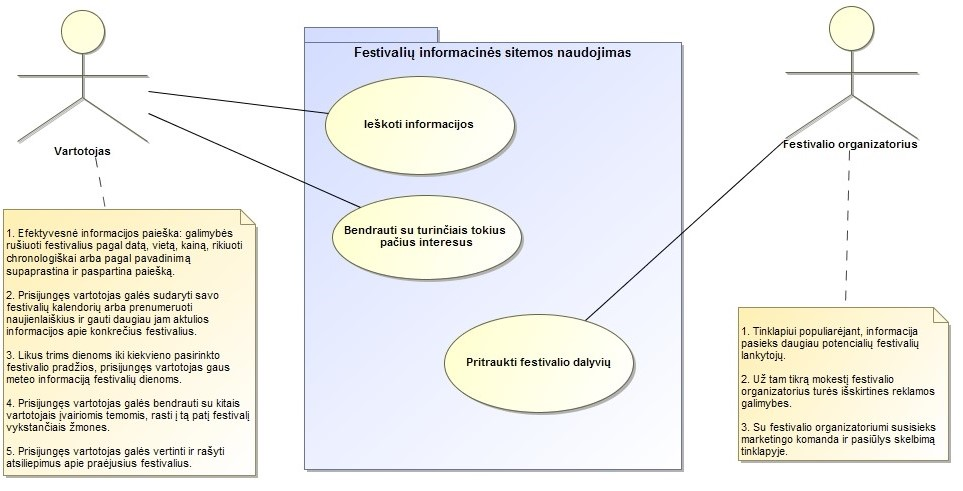
\includegraphics[scale=0.5]{img/geri/sisNauda}
    \label{img:uml28}
	\caption{Sistemos teikiamos naudos diagrama}
\end{figure}

\subsection{Esama būklė}
\begin{itemize}
	\item 4 kompiuteriai
	\item 4 žmonės
\end{itemize}

\subsection{Priemonės scenarijui įgyvendinti}
\begin{itemize}
\item Serverio nuoma - tinklapio talpinimui, dėl padidėjusio lankytojų skaičiaus senas serveris gali būti netinkamas;
\item Duomenų bazė - talpinama informaciją apie fesitvalius, vartotojų informaciją (prisijungimo duomenys, komentarai ir pan.), straipsnius.
\item “Microsoft Office” licencija - straipsnių rašymui ir buhalterijos vedimui;
\item “Photoshop” licencija - į tinklapį keliamų nuotraukų redagavimui;
\item Verslo liudijimas - legaliam reklamos erdvės tinklapyje pardavimui;
\item Facebook reklamos - sistemos populiarinimui;
\item Žmogiškieji ištekliai:
    \begin{itemize}
    \item Programuotojų paslaugos - naujų funkcijų kūrimui ir diegimui;
    \item Marketingo komanda - sistemos populiarinimui, komunikacijai su festivalių organizatoriais;
    \item Administratoriai - sistemos tvarkai palaikyti;
    \item Žurnalistas - straipsnių rašymui.
    \end{itemize}
\end{itemize}

\section{Įgyvendinamumo ir naudos analizė}
\subsection{Operacinis įgyvendinamumas}
\begin{longtable}{|p{0,45\linewidth}|p{0,45\linewidth}|}
\caption{Operacinis įgyvendinamumas}\\
	\hline
	Inovacinis slenkstis & Inovacinio slenksčio pašalinimas\\
	\hline
	Festivalių informacinė sistema nėra žinoma tarp potencialių lankytojų. &
	Reklamuoti socialiniuose tinkluose.\\
	\hline
	Lankytojai nežino visų tinklalapio galimybių ir kaip jomis naudotis. &
	Informuoti lankytojus. Užsiregistravusiems vartotojams, kartu su registracijos patvirtinimu, į elektroninį paštą atsiųsti detalų visų galimybių aprašymą bei kaip jomis pasinaudoti. Sukurti vartotojui lengvai suprantamą vartotojo sąsają. Puslapyje pateikti informacinį elektroninio pašto adresą ir atsakyti į vartotojams kylančius klausimus.\\
	\hline
	Festivalių informacinė sistema nėra žinoma tarp festivalių organizatorių. & Susisiekti su festivalių organizatoriais.\\
	\hline
\end{longtable}
\subsection{Techninis įgyvendinamumas}
Mūsų kuriama sistema nėra visiškai nauja idėja. Analizės metu mes apžvelgėme panašią egzistuojančią sistemą, tačiau mūsų sistema būtų labiau išbaigta ir turėtų daugiau funkcijų. Sistemos funkcijoms įgyvendinti reikia tinklalapio ir duomenų bazės, kurie galėtų būti patalpinti viename serveryje. Duomenų bazėje lentelėse būtų talpinama informacija apie festivalį, komentarus ir vartotojų informaciją.

Susikurdami tinklalapio paskyrą vartotojai turės užpildyti paskyros laukelius, o prisijungdami per socialinius tinklus už vartoją bus pasirūpinta tų laukelių užpildimu ir naujos paskyros tinklalapyje sukūrimu.
\subsection{Ekonominis įgyvendinamumas}
\subsubsection{Išlaidos}
 
Mūsų tinklalapis talpins informacija apie festivalį, todėl mums reikės serverio ir domeno. Serverio kainos svyruoja nuo 1€ iki 30€, domeną galima nusipirkti už 8€ .
Mūsų tinklalapį aptarnaujančią komandą sudaro administratoriai, žurnalistai ir marketingo komanda. Tikėtina, kad mėnesinis atlyginimas administratoriui sieks 600€ (+ 240€ mokesčių),  žurnalistui ir marketingo komandos nariui po 400 (+160€). Tikriausiai turėsime po vieną kiekvienos komandos narį.  Norint išpopuliarinti tinklalapį, reikėtų užsakyti reklama “Facebook” tinke. Per diena ketiname išleisti apie 10€ reklamai. Tinklalapį kuriantiems programuotojams mokėtumėme 1500€, tikėdamiesi kad jie pilnai sukurs sistemą per 3 mėnesius.
 
Pradinės išlaidos: 4500€
 
Mėnesinės išlaidos: 2038€ (1400€ atlyginimas + 560€ mokesčiai +60€ reklama +18€ tinklalapio išlaikymas)
 
\subsubsection{Pajamos}
 
Mūsų tinklalapis pajamas generuos parduodamas išskirtinę reklamą festivalių organizatoriams ir prašydamas vartotojų skirti 2\% nuo pajamų mokesčių. Tikėtina kad reklama pirmuoju laikotarpiu kainuos 30€ /mėn ir turėsim tik vieną reklamos pirkėją. Tinklalapiui išpopuliarėjus kaina pakils iki 10€ / dienai ir turėsime 3 reklamos pirkėjus. 2\% mokesčių nuo vidutinio darbo užmokesčio siekia apie 3,5€. Pradžioje planuojame turėti 5 paramos skyrėjus, o išpopuliarėjus - apie 100 skyrėjų.
 
Mėnesinės pajamos:
 
Pradėjus veiklą: 45€
 
Išpopuliarėjus: 1250€
 
Mes sieksime gauti Europos sąjungos finansavimą. Galvojame pateikti užklausą projektui - Ekologinio (pažintinio) turizmo, aktyvaus poilsio ir sveikatos gerinimo infrastruktūros kūrimas ir plėtra. Mes teigtume, kad mūsų tinklalapis, turėdamas visą reikalingą informaciją apie festivalius Lietuvoje, paskatins žmones aktyviai praleisti savo laisvalaikį ir ilgalaikiu požiūriu gali pritraukti turistus į Lietuvą dėl kultūrinių ir kokybiškų festivalių. Tai gali padidinti miestų, kuriuose vyksta festivaliai, įplaukas.
\subsection{Juridinis Įgyvendinamumas}
 Mūsų kuriamai sistemai svarbiausias juridinis klausimas yra - ar nebus pažeistas asmens duomenų teisinės apsaugos įstatymas. Mūsų sistemos funkcionalumas ir tikslai nepažeidžia asmens duomenų apsaugos įstatymo tikslo - “ginti žmogaus privataus gyvenimo neliečiamumo teisę tvarkant asmens duomenis”. Mūsų sistema registracijos metu prašo tik susisiekimui reikalingų duomenų (elektroninio pašto) ir vartotojui kuriantis paskyrą bus prašoma įvesti jo paties sugalvotą slapyvardį, kuris bus naudojamas jo identifikacijai, taip nuslepiant jo tikrąją tapatybę. Iš socialinių tinklų (jeigu vartotojas nuspręs registruotis per juos) tinklalapis ims tik paskyrai sukurti reikalingą informaciją.
%\printbibliography[heading=bibintoc] 
\section{Žodynas}
\begin{sortedlist}
  \sortitem{Sistemos savininkas - fizinis arba juridnis asmuo, kuriam priklauso turtas (tinklalapis).}
  \sortitem{Tinklalapis - informacijos šaltinis žiniatinklyje (internete), kuris gali būti pasiektas naudojantis naršykle.}
  \sortitem{Festivalio puslapis - tinklapio skiltis, kurioje patalpinta vieno festivalio informacija.}
  \sortitem{Vartotojas - asmuo, kuris tiesiogiai naudojasi (tinklalapio) paslaugomis.}
  \sortitem{Registruotas vartotojas - vartotojas, užsiregistravęs tinklapyje.}
  \sortitem{Administratorius - sistemos savininko įgaliotas asmuo, kuris prižiūri tinklalapį ir turi priėjimą prie specialių tinklalapio funkcijų.}
  \sortitem{Festivalio organizatorius - asmuo arba įmonė, kuri rengia renginį (festivalis).}
  \sortitem{Festivalių duomenų bazė (FDB) - organizuotas duomenų rinkinys, kuriame yra talpinama festivalių informacija.}
  \sortitem{Serveris - kompiuteris, pasiekiamas internete, kuris priima užklausas iš kitų kompiuterių ir pateikia atitinkamus atsakymus ar rezultatus.}
  \sortitem{Socialinis tinklas – interaktyvi interneto struktūra (interneto svetainė), vienijanti tam tikrą, bendrų interesų turinčią narių grupę, kuri ir kuria konkrečios svetainės turinį ir virtualiai bendrauja tarpusavyje, automatizuotomis konkrečios svetainės priemonėmis.}
  \sortitem{Socialinių tinklų įskeipis - tinklalapio dalis, kuriame galima dalintis arba išreikšti savo nuomonę naudojantis socialiniais tinklais.}
  \sortitem{“Facebook” komentarų erdvė - vieta, kurioje elektroniniu būdu (rašydamas) vartotojas (su Facebook paskyra) gali reikšti savo nuomonę.}
  \sortitem{Informacija apie festivalį - anketa, kuri yra užpildoma norint talpinti informaciją į  FDB.}
  \sortitem{Festivalis - masinė kultūros (paprastai periodiška ir trunkanti kelias dienas) šventė.}
  \sortitem{Marketingo komanda - asmenys, kurie tarpininkauja tarp festivalių organizatorių ir tinklapio administratoriaus, rūpinasi tinklapio reklama.}
  \sortitem{Komentarų erdvė - puslapio sritis, kurioje yra rodomi komentarai, o prisijungę vartotojai turi galimybę skelbti savo komentarus.}
  \sortitem{Dalykinė sritis – sritis, kurioje naudojama sistema.}
  \sortitem{Vietinė tinklalapio paskyra - paskyra, sukurta pačiame tinklalapyje.}
  \sortitem{Interaktyvumas - vartotojų dalyvavimas, komunikacija, turinio kontrolė.}
  \sortitem{Domenas – interneto svetainės adresas (pvz.: dom.lt) ir el. pašto adreso kamienas (pvz.: info@dom.lt).}
  \sortitem{Juridinis - teisinis, susijęs su teise; turintis teisę valdyti turtą, sudaryti sutartis.}
\end{sortedlist}

\sectionnonum{Literatūros sąrašas}
\begin{itemize}
\item http://manofestivalis.lt/
\item https://www.facebook.com/ManoFestivalis.lt/?fref=ts
\item https://www.e-tar.lt/portal/lt/legalAct/TAR.5368B592234C/lGOrBAvuZc (Lietuvos Respublikos asmens duomenų teisinės apsaugos įstatymas)
\item https://www.esparama.lt
\item https://www.vmi.lt/ (2\% nuo pajamų mokesčio parama)
\item http://www.hostingas.in/
\item http://jobarnesonline.com/free-facebook-ad-spend-calculator/
\item https://www.tutorialspoint.com/uml/uml\_2\_overview.htm
\item http://www.mif.vu.lt/\textasciitilde karolis/PSI1.html
\end{itemize}

%\appendix  % Priedai
% Prieduose gali būti pateikiama pagalbinė, ypač darbo autoriaus savarankiškai
% parengta, medžiaga. Savarankiški priedai gali būti pateikiami ir
% kompaktiniame diske. Priedai taip pat numeruojami ir vadinami. Darbo tekstas
% su priedais susiejamas nuorodomis.

%Citavimo pavyzdžiai: cituojamas vienas šaltinis \cite{PvzStraipsnLt}; cituojami
%keli šaltiniai \cite{PvzStraipsnEn, PvzKonfLt, PvzKonfEn, PvzKnygLt, PvzKnygEn,
%PvzElPubLt, PvzElPubEn, PvzMagistrLt, PvzPhdEn}.
%
%
%\subsubsection{Skirsnis}
%\subsubsubsection{Straipsnis}
%\subsubsection{Skirsnis}%

\end{document}
